\chapter{Chapter 2 Design and Implementation}

% \begin{chapterabstract}
%     Use the chapterabstract environment, not the abstract environment, if you want to plant an abstract at the top of the chapter.
% \end{chapterabstract}


% \begin{quote}
% If needed Here's a quote environment.
% \end{quote}


% Here's a citation, so we don't get a "no citation warning" \cite{GolV13}. Here's a figure.
% \begin{figure}
%     \begin{centering}
%         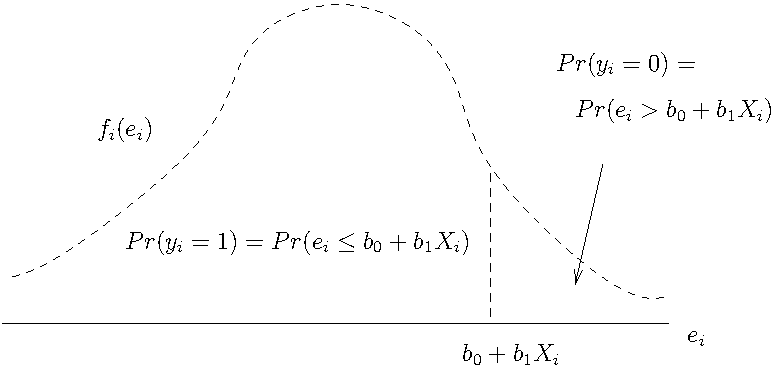
\includegraphics[scale=0.8]{design/chap_1_figures/example_1.pdf}
%     \par\end{centering}
%     \caption{Figure for list of figures  in the content page.}
%     \label{fig:first_fig}
% \end{figure}
% Here how to reference a figure such as Figure \ref{fig:first_fig}.
% \newpage

% \includestandalone[width=.8\textwidth]{chap_1_figures/State}

\section{Smart Contract Object Model}


\subsection{Types of Items}


The data model for the smart contract is designed around the key-value interface of the ledger and the fabric stubs  ability to store the state of object under composite keys. The composite keys support querying the world state by levels of hierarchal keys that are appended onto each other. The definition of the objects are done though a protobuf definition file, where the objects are messages that have been annotated with the KeySchema option message.
% refracing needed here

The objects that are managed by the smart contract are grouped into two sets primary objects and sub-item types. The primary objects are the objects types that are directly managed by the access control and the sub-items are used to manage metadata and auxiliary state of the primary objects. In the proof of concept implementation the two sub-item that are defined are the Hidden Transaction list and the Suggested Updates.


%  Definitions of the keys
All of primary objects have to have a collection Id property and then have the paths to the properties that make up the other attributes of the key listed in the key FieldMask property of the annotation.


\subsection[short]{Stages of Generic Object Contract}
The smart contract is broken up into three stages. The first stage is responsible for defining functions that are exposed by the smart contract. This layer is responsible for initial validation and unpacking the requests arguments provided to the invocation of the smart contract. It is also responsible for calling the second stage function and then packing the item into its return format. The second stage is a wrapper around the fabric shim interface to the world state that defines defines the operations that can happen on primary objects and their sub-object domains. This layer is responsible for building the operation data structure by setting the action field biased on the function and then extracting the collection id, the type of the object, and potentially the paths that the action takes place on from the object and arguments passed into the function. This operation is then handed of to the third and final stage where the action is authorized. If the operation is authorized the second layer then calls the required chaincode stub functions to interact with the ledger.



\begin{table}

    \centering                       % Center your table

    \begin{tblr}
        {
            hline{1,Z} = {2pt},
            hline{2} = {1pt},
            hline{3-Y} = {},
            vline{1,Z} = {},
        }
             % Your table
        Function                   & Transaction Type & Action          \\
        Get                        & Query            & View            \\
        List                       & Query            & View            \\
        ListByCollection           & Query            & View            \\
        ListByAttrs                & Query            & View            \\
        Create                     & Invoke           & Create          \\
        Update                     & Invoke           & Update          \\
        Delete                     & Invoke           & Delete          \\
        GetHistory                 & Query            & View History    \\
        GetHiddenTx                & Query            & View Hidden Txs \\
        HideTx                     & Invoke           & Hide Tx         \\
        UnHideTx                   & Invoke           & UnHide Tx       \\
        GetSuggestion              & Query            & Suggest View    \\
        SuggestionListByCollection & Query            & Suggest View    \\
        SuggestionByPartialKey     & Query            & Suggest View    \\
        SuggestionCreate           & Invoke           & Suggest Create  \\
        SuggestionDelete           & Invoke           & Suggest Delete  \\
        SuggestionApprove          & Invoke           & Suggest Create
    \end{tblr}
	\caption{Functions In Generic Collection Smart Contract}           % Caption
	\label{tab:my-first-table}       % Label
\end{table}